\section{Specific distinction and retained support}
\label{sec:specific-distinction}
\label{sec:introduction}
\label{sec:afc-basis}

\subsection{Premises and scope}
\label{subsec:intro-aim-stance}
\label{subsec:intro-scope}
\label{subsec:afc-null-potential}
AFC begins with Null potential, expressed as Null sameness: a finite distinction supplies the relata of a
relation. A\(\Omega\)D takes the primitive distinction to have retained
branch, hinge and counterbranch roles. Its completed return is one closure
phase. The construction repeats at every admitted finite scale. These are
the foundation and scope of the ontology developed here; transition weights,
duration accessors and response laws are declared after the relations they use.

\label{subsec:null-presentation}
\begin{equation}
x=\Null,\qquad x=x,\qquad \Null\equiv\infD.
\label{eq:null-axiom}
\end{equation}
Here \(\infD\) names undifferentiated potential, with no finite coordinates,
ordered events or probability space already assigned to it. The notation
\begin{equation}
\Null\equiv\infty,\qquad \Null\to\Null\to\Null\equiv\Null
\label{eq:null-presentation}
\end{equation}
is an identity presentation of that sameness. A displayed repetition of its
glyph is a notation, not a previously indexed Null history.

\paragraph{AF scope.}
\label{subsec:intro-use}
A distinction induces its retained relation; certified returns support
recurrence, scoped organization, model values and their projections.
The finite calculus names curl, monon, dion, duon, curling support, shell,
reflection-duration coupling, pressure, SADAR, Fractal Field Ring Gate (FRG), fusion and sheddic routing at
their respective types. The Art of the Leprechaun is the tracing and exploration of Stokes temporal wave dynamics through retained cuts and recurrent forms. The Manual carries worked
models and calibrated comparisons with their declared domains.

\subsection{First finite anchor}
\label{subsec:afc-fractal-address}
The first distinction co-creates its start and finite addressability. Write
its inevitable anchor as
\begin{equation}
a_0=\mathtt{00}_8,\qquad
\mathbf a\in\mathcal A^{\mathrm{ret}}_8
\subseteq\{0,1,\ldots,7\}^{<\omega}.
\label{eq:first-anchor}
\end{equation}
The octal notation is an encoding of retained address, with displayed ladder
\(\mathtt{00}_8,\mathtt{01}_8,\ldots,\mathtt{07}_8,\mathtt{10}_8,\ldots\).
It does not choose a start from prior finite coordinates. Below this first
anchor the finite construction is unbound. Null, fibre zero, the binary
vertex \(0000\), octal anchor \(\mathtt{00}_8\), and its scope \(B_0\)
are five distinct types. The left glyph \(a\mid-\) binds a retained address;
\(0\mid-\) is its local origin notation.

\subsection{Branch, hinge and counterbranch}
\label{sec:cut-running-fractal-tesseract}
\label{subsec:null-symmetry}
\label{subsec:cut-running}
The distinguished running relation is
\label{subsec:local-cut-running-form}
\begin{equation}
x\longmapsto x\succ x=x.
\label{eq:cut-running-form}
\end{equation}
The equality records return to the retained start only when the trace and
closure witness below are supplied. The compact grammar and its expansion are
\label{subsec:branch-hinge-branch}
\begin{equation}
1\,0^*\,-1
\quad\rightsquigarrow\quad
M_{\varepsilon,m}=\varepsilon\,0_H(0_D)^m(-\varepsilon),
\qquad \varepsilon\in\{-1,+1\},\quad m\in\mathbb Z_{\ge0}.
\label{eq:hinge-grammar}
\end{equation}
The hinge \(0_H\) is structural; the star permits additional dwell \(0_D\).
Thus \(m=0\) retains the hinge. The two branches and the hinge belong to one
distinction construction. Interior, boundary and exterior are induced sided
roles of that construction, rather than separately assembled primitive cuts.

\paragraph{Oriented reflection.}
The distinction has oriented sides \(\mathrm{me}\mid\mu\mid\text{not-me}\).
Reflection exchanges their branch roles and retains the hinge:
\begin{equation}
\iota(\mathsf H_3^{\varepsilon})=\mathsf H_3^{-\varepsilon},\qquad
\iota(\mu)=\mu,\qquad\iota^2=\mathrm{id}.
\label{eq:hinge-reflection-involution}
\end{equation}
This is an involution of the sided construction, before assigning temporal
crown roles or choosing a weighted continuation model.

\paragraph{Retained roles.}
\label{subsec:hinge-triad}
At a committed crown \(k\), write
\begin{equation}
\mathsf H_3^{\mathrm{role}}(k)=(x_k^-,\mu_k,\mathcal H_k^+),\qquad \mu_k=x_k^0.
\label{eq:hinge-triad}
\end{equation}
The roles are retained predecessor, present crown and admitted successor
horizon \(\mathcal H_k^+\). A committed continuation selects a member
\(h_k^+\in\mathcal H_k^+\). The same hinge-mediated relation applies at \(k=0\), at arbitrary
\(k\), and at a newly admitted enclosing scale. Its universality follows from
applying the one construction rule at each admitted occurrence; a finite
enumeration supplies witnesses, not a replacement premise.

\subsection{Faithful atomic encoding}
\label{subsec:fractal-tesseract}
\label{subsec:fractal-recursive-support}
\label{subsec:four-edge-x-witness}
\label{subsec:q4-four-edge-implementation}
A faithful atomic encoding changes exactly the coordinate that records the
one retained distinction. In the finite tesseract witness,
\begin{equation}
V(\Qfour)=\{0,1\}^4,\qquad
E(\Qfour)=\{(u,v):d_H(u,v)=1\},\qquad
d_H(u,v)=\#\{j:u_j\ne v_j\}.
\label{eq:atomic-h1}
\end{equation}
For any admitted atomic event at any retained scale, all other encoded
coordinates are unchanged and the distinguished coordinate differs; hence
\(d_H=1\). This argument is independent of the number of other coordinates.
Two consecutive H1 steps may have an H2 composite endpoint. A nontrivial
closed H1 word has endpoint distance zero while retaining every traversal.

\paragraph{Ancestor support.}
\label{subsec:four-edge-ancestor}
Each \(\Qfour\) vertex has four incident edges. At a retained occurrence one
slot binds the ancestor and three other slots remain available for the declared
continuation. This is an incidence statement. A certified closure may use a
two-edge return or a longer even word. It is not required to traverse all four
incident edges. Recursive occurrences retain the same ancestor distinction.

\begin{figure}[H]
\centering
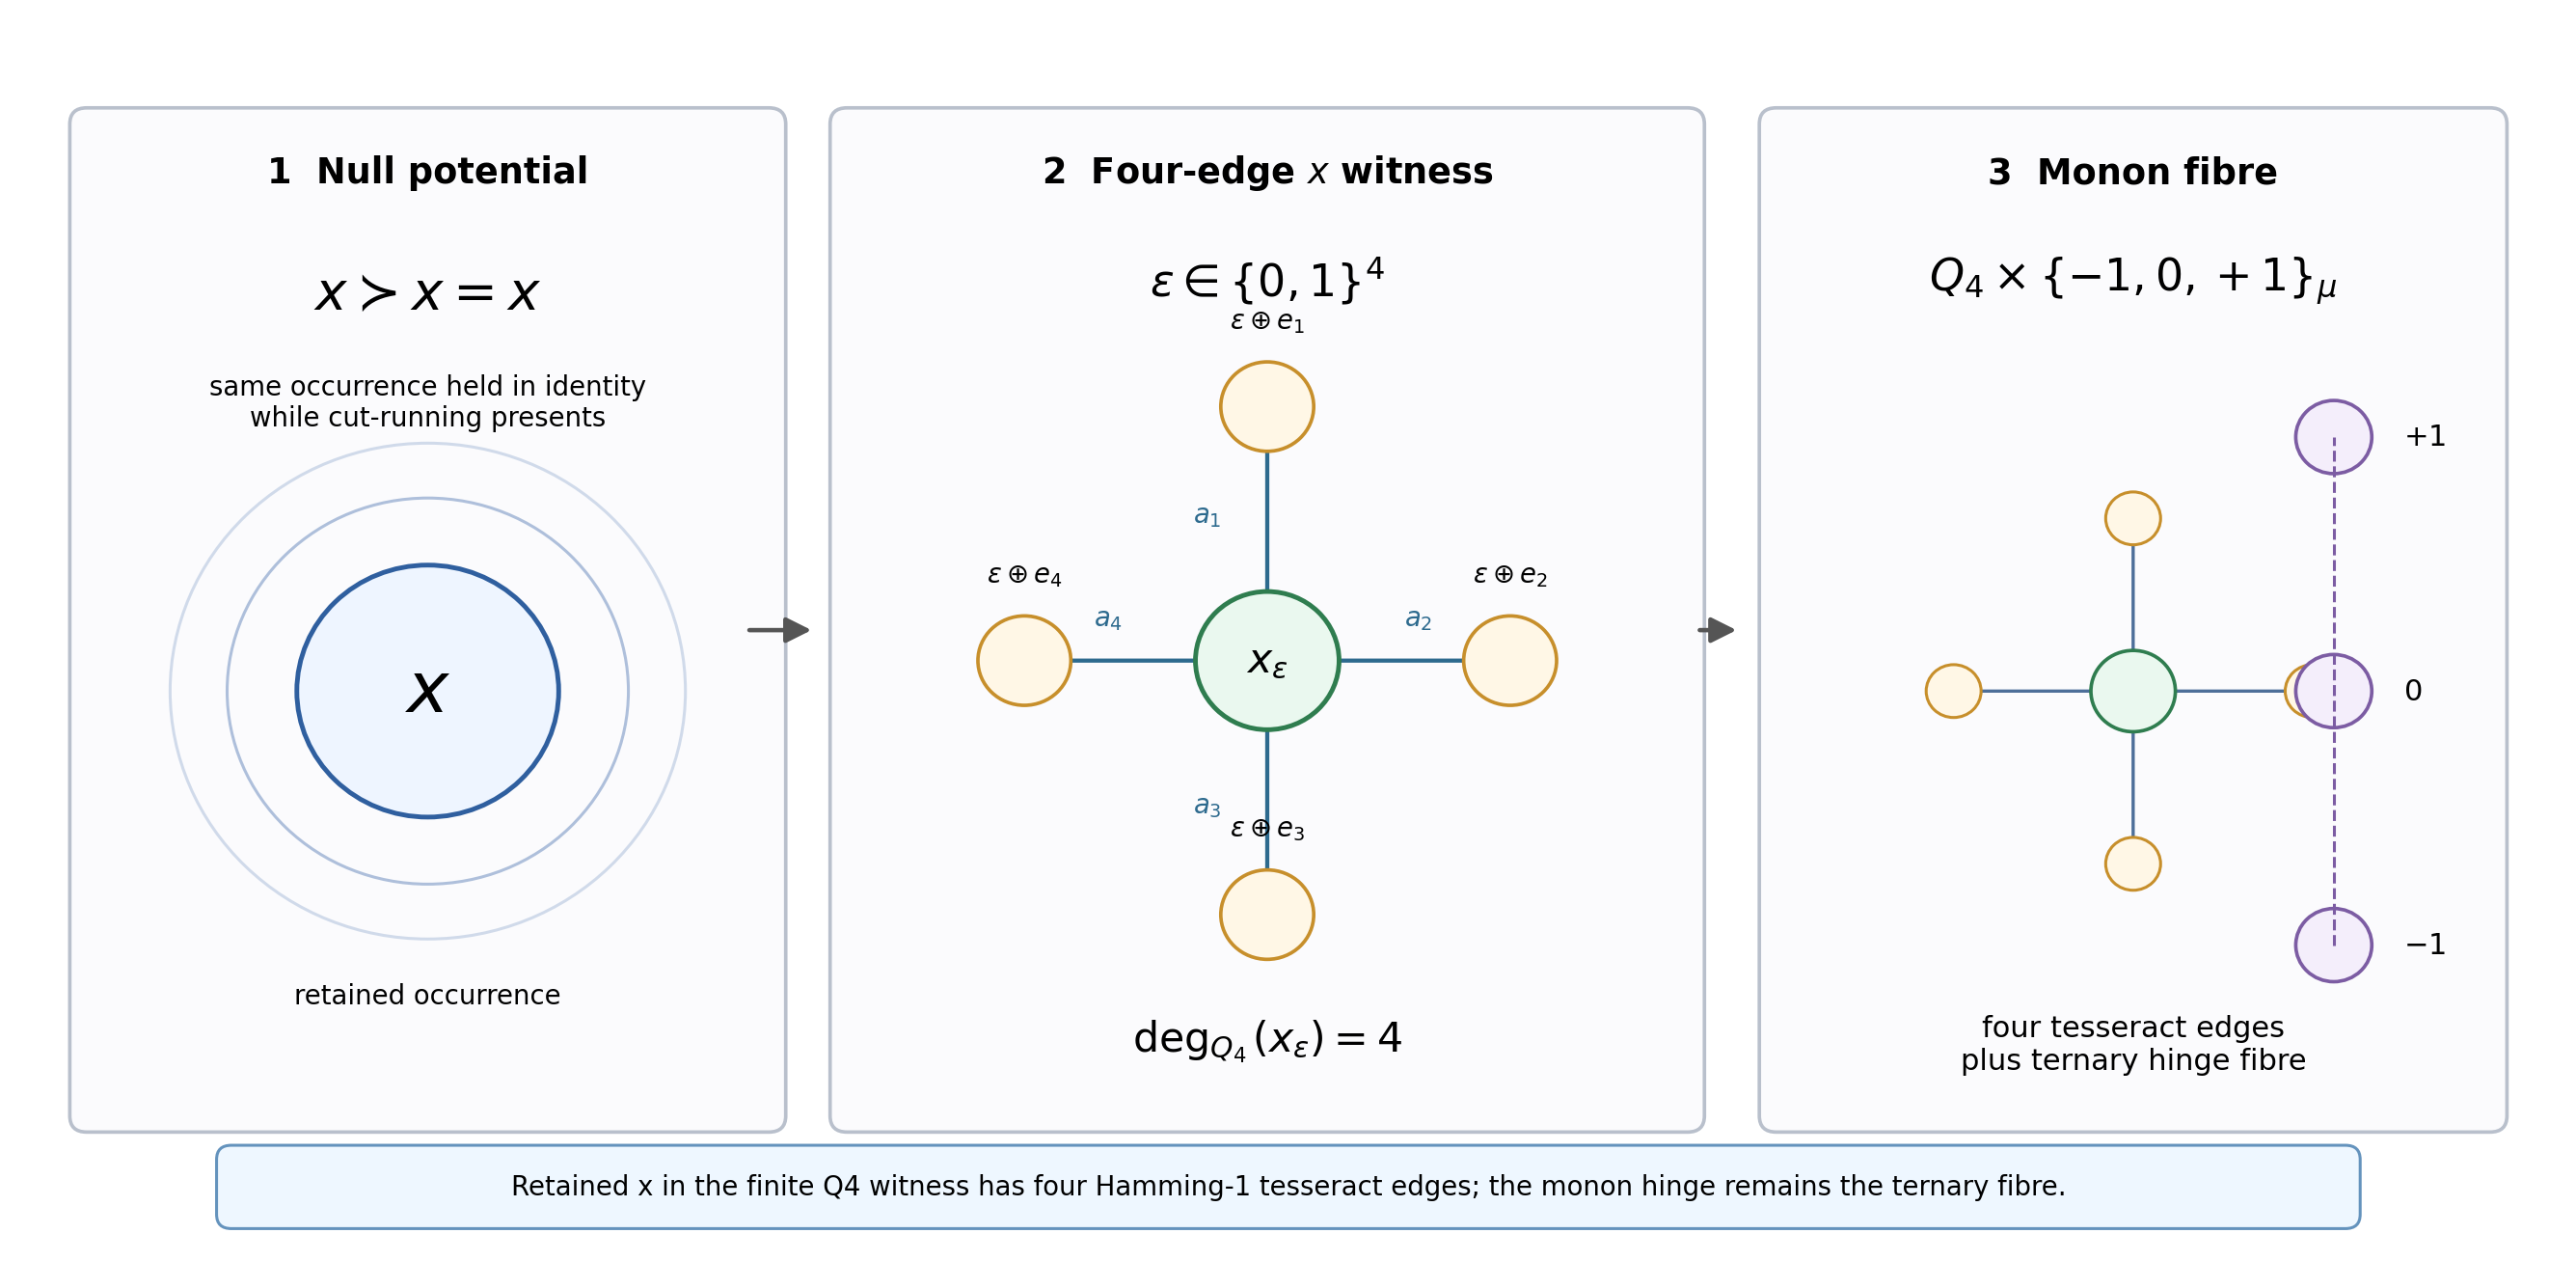
\includegraphics[width=0.72\linewidth]{figures_jpg/null_four_edge_x_witness.png}
\caption{Finite four-edge encoding of a retained occurrence. The vertex is a
post-distinction witness; Null itself has no vertex address.}
\label{fig:null-four-edge-x-witness}
\end{figure}
\begin{figure}[H]
\centering
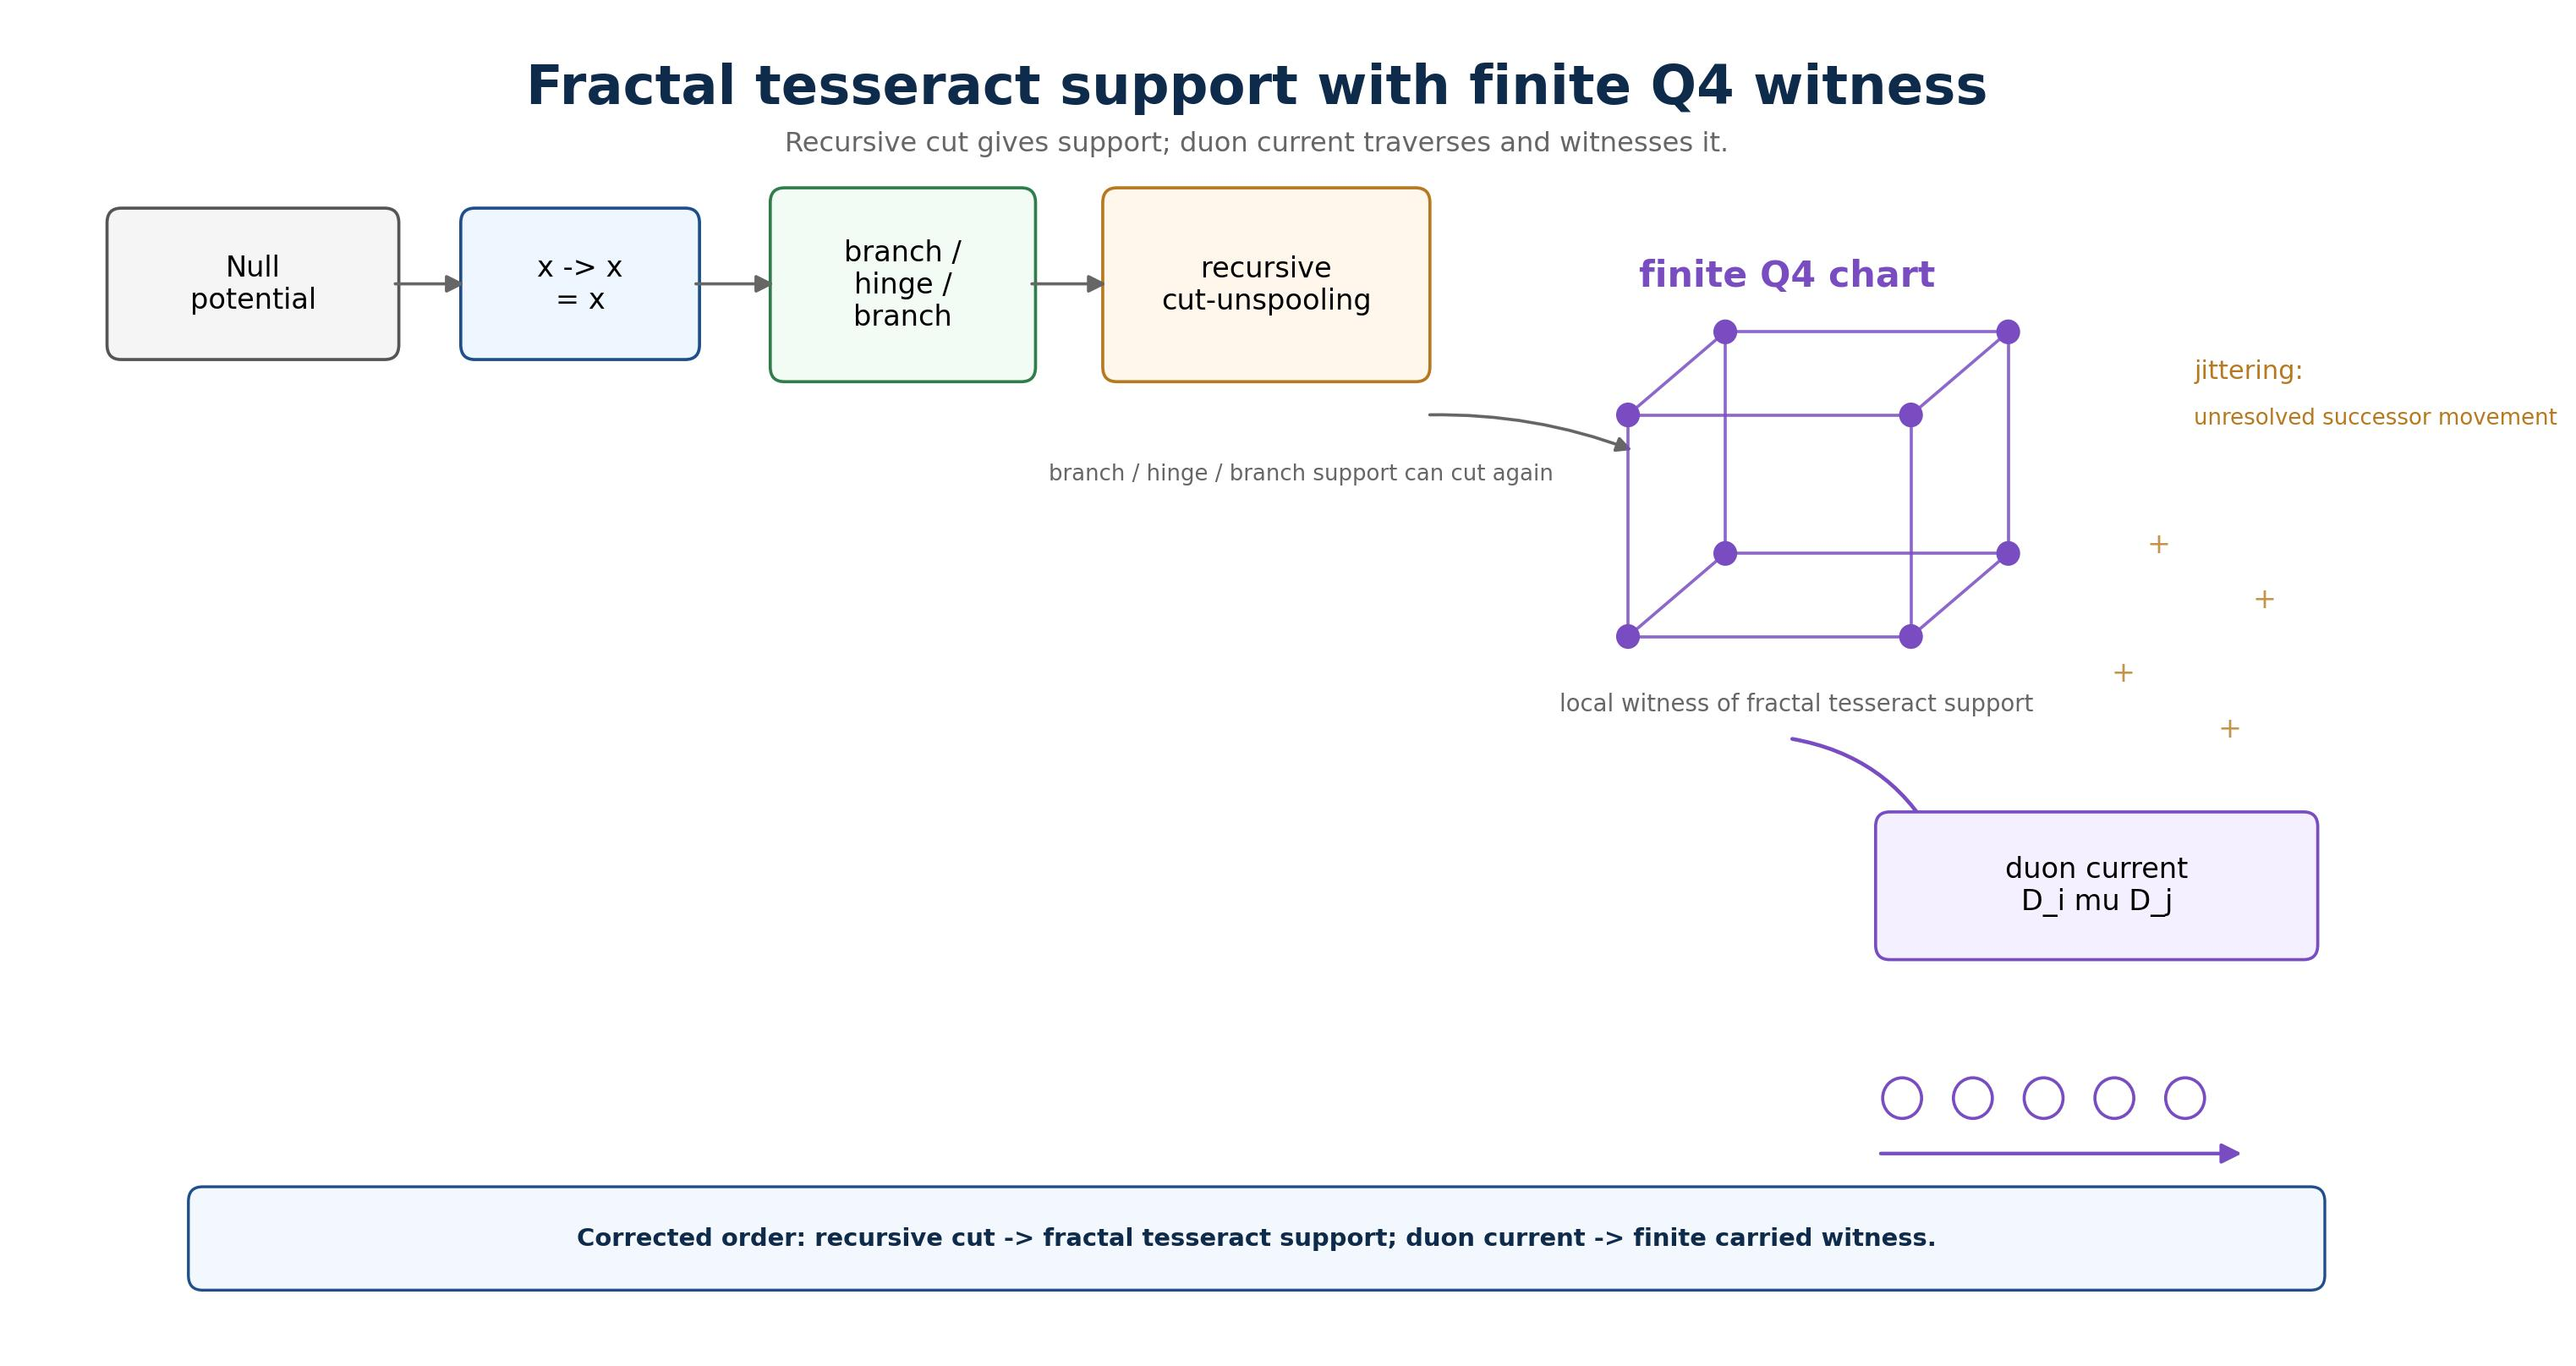
\includegraphics[width=0.72\linewidth]{figures_jpg/fractal_tesseract_q4_witness.jpg}
\caption{The finite tesseract support. Local degree and total closure-word
length are distinct quantities; oriented ancestry remains in the trace.}
\label{fig:v39-fractal-tesseract-q4-witness}
\end{figure}

\paragraph{Conditional support.}
\label{subsec:ternary-capacity}
Every probability measure later declared on a nonempty admitted atomic
support is concentrated on H1 events, because every element of that support
satisfies \eqref{eq:atomic-h1}. Consequently
\begin{equation}
\Pr[d_H=1\mid\text{admitted atomic event}]=1.
\label{eq:atomic-probability-one}
\end{equation}
This conditional support statement supplies neither a prior probability on
Null nor a probability-one closure theorem. Ternary assignment capacity is
the separate finite information count
\begin{equation}
C_3(k)=\log_3(3^k)=k.
\label{eq:ternary-capacity}
\end{equation}

\subsection{Common retained records}
\label{subsec:afc-boundary-accounting}
A scope \(B=(\partial_T R,\omega)\) binds an induced retained interface and
a finite committed comparison window. Write \(\mathbf a\vdash(R,\partial_T
R,\omega)\) when the address must be explicit. Each event has immutable
identity, lineage, scope, scale, predecessor, role and committed order.
The trace prefix consists of those events in that order. A construction
record binds its exact prefix digest and witness; validation checks those
bindings against the declared registry. A record validates a construction
already made and cannot originate its distinction or recurrence.


\begin{equation}
\partial_T R\subseteq E(\Qfour)\times\{-1,0,+1\},
\qquad B=(\partial_T R,\omega).
\label{eq:tesseract-admissible-boundary}
\end{equation}
The finite base and the ternary role fibre are different coordinates. A fibre
hinge can be present without a new base traversal.

\paragraph{Falsification.}
An advertised atomic H2 edge, missing retained ancestor, hinge bypass or
pre-existing finite origin contradicts the stated construction. A lawful
composite H2 endpoint and a closure endpoint at H0 do not contradict atomic H1.

\paragraph{Provenance.}
AFC, Axioms (Null and distinction-induced relations), anchors \texttt{ax:null-infinity}, \texttt{cons:region}, \texttt{cons:relations}; Choices (finite
retained support); A\(\Omega\)D's branch/hinge/counterbranch and first-anchor
construction. Binary hypercube encoding is a finite realization of the declared
atomic distinction rule. Later weighted kernels use this support.
\aodliteraturenote{Finite graph and walk context: Norris~\cite{norrisMarkov},
Levin--Peres--Wilmer~\cite{levinPeresWilmer},
Lawler--Limic~\cite{lawlerLimic}.}

\paragraph{Exact arithmetic.}
\label{subsec:radical-free-arithmetic-policy}
Native decisions use finite integer and rational sums, products, signs,
orders, ratios and declared finite powers. Exact finite characters are
downstream representation coordinates. Calibrated geometry and empirical
comparison maps have their own Manual scope.
